% !TeX Options = -shell-escape

\documentclass[10pt]{beamer}

\usetheme[progressbar=frametitle, block=fill]{metropolis}
\usepackage{xcolor}
\usepackage{multirow}
\usepackage{pgfpages}
\usepackage{pifont}
\usepackage[utf8]{inputenc}
\usepackage[T1]{fontenc}
\usepackage{csquotes}
\usepackage[english]{babel}
\newcommand{\cmark}{\ding{51}}
\newcommand{\xmark}{\ding{55}}
\setbeamertemplate{note page}{\insertnote}
%\setbeameroption{show notes on second screen=left}
\setbeameroption{hide notes}
\definecolor{amethyst}{rgb}{0.5, 0.4, 1.0}
\definecolor{amethystgrey}{rgb}{0.85, 0.85, 1.0}
\definecolor{amethystdark}{rgb}{0.4, 0.3, 0.9}
\definecolor{orangedark}{rgb}{0.0, 0.9, 0}
%\definecolor{titlebg}{HTML}{4e8074}
%\definecolor{titlebg}{HTML}{3e7985}
\definecolor{titlebg}{HTML}{fbf8ff}
\definecolor{font}{HTML}{23373b}
%\setbeamercolor{title}{fg=amethyst, bg=amethyst}
\setbeamercolor{frametitle}{fg= font, bg=titlebg}
%\setbeamercolor{section title}{black}
%\setbeamercolor{structure}{fg=amethyst, bg=amethyst}
\setbeamercolor{progress bar}{ fg = amethyst, bg= amethystgrey }
%\setbeamercolor{itemize item}{fg=amethyst,bg=white}
\setbeamercolor{alerted text}{fg=amethystdark}
%\setbeamercolor{title separator}{ ... }
%\setbeamercolor{progress bar in head/foot}{ ... }
%\setbeamercolor{progress bar in section page}{ ... }

\usepackage{booktabs}
\usepackage[scale=2]{ccicons}

\usepackage{minted}

\usepackage{pgfplots}

\usepackage{xspace}

\title{C++ 14}
\subtitle{complete feature description}
\date{}
\author{Dawid Pilarski}
\institute{dawid.pilarski@panicsoftware.com \\ blog.panicsoftware.com}

\begin{document}

\maketitle

\section{Introduction}
\begin{frame}{C++ 14}
	\begin{columns}[T]
		\begin{column}{0.48\linewidth}
				Language changes 
				\vskip0.5em
					\hrule
			\begin{itemize}
				\item \alert{type deduction}
				\item \alert{better lambdas}
				\item \alert{variable templates}
				\item \alert{relaxed constexpr}
				\item \alert{binary literals}
				\item \alert{non const constexpr functions}
				\item \alert{deprecated attribute}
				\item \alert{member initializers and aggregates}
				\item \alert{sized deallocations}
				\item \alert{digit separation}
				\item \alert{contextual conversions}
			\end{itemize}
		\end{column}
		\begin{column}{0.48\linewidth}
				Library changes 
				\vskip0.5em
					\hrule
			\begin{itemize}
				\item \alert{ud literals extended}
				\item constexpr for STL
				\item std::quoted
				\item null forward iterators
				\item std::result\_of SFINAE-friendly
				\item std::shared\_timed\_mutex
				\item std::get<T>()
				\item integral\_constant as a functor
				\item \alert{std::index\_sequence}
				\item std::exchange
				\item std::equal, std::is\_permutation, std::mismatch
			\end{itemize}

		\end{column}	
	\end{columns}
\end{frame}

\begin{frame}{Who am I?}
			\centering \alert{Dawid Pilarski}
			\vskip 1em
	\begin{columns}[onlytextwidth]
		\begin{column}{0.7\textwidth}
			\begin{itemize}
				\item Senior Software Developer in TomTom
				\item Member of the ISO/JTC1/SC22/WG21
				\item Member of the PKN KT {\tiny(programming languages)}
				\item MENSA member
				\item C++ blog writer
			\end{itemize}
		\end{column}
		\begin{column}{0.29\textwidth}
				
\includegraphics[width=\linewidth]{Dawid_Pilarski.jpg}				
		\end{column}	
	\end{columns}
\end{frame}

\section{Language changes}
\section{Type deduction}
\begin{frame}[fragile, label=typeDeduction]{Type deduction}
	\centering we could deduce the returned type in C++ 11:

	\begin{minted}{c++}
template <typename T>	
auto sum(T a, T b) -> decltype(a+b){
  return a + b;
}
	\end{minted}

	\pause

	\begin{alertblock}{The issue in C++ 11}
	a + b is now a code repetition!
	\end{alertblock}

\end{frame}

\begin{frame}[fragile]{Return type deduction}
	\centering \alert{\Large C++14} \\ 
	\vskip 1em
	 How to avoid the code repetition?

	\begin{columns}
		\begin{column}{0.48\linewidth}
	\begin{minted}{c++}
template <typename T>	
auto sum(T a, T b){
  return a + b;
}
	\end{minted}
		\end{column} \pause 
		\begin{column}{0.48\linewidth}
\begin{minted}{c++}
template <typename T>
decltype(auto) sum(T a, T b){
  return a + b;
}	
\end{minted}
		\end{column}
	
	\end{columns}
\end{frame}

\begin{frame}[fragile]{Where can we use deduction?}

	\begin{onlyenv}<1-2>
		\begin{itemize}
			\item \alert{for regular functions}
		\end{itemize}

		\vfill
	\end{onlyenv}

	\begin{onlyenv}<1>
		\begin{minted}{c++}
struct A {
  auto f(); // forward declaration
};
auto A::f() { return 42; }
\end{minted}
	\end{onlyenv}
	\begin{onlyenv}<2>
	\begin{minted}{c++}
auto f(); // return type is unknown
auto f() { return 42; } // return type is int
auto f(); // redeclaration
int  f(); // error, declares a different function	
	\end{minted}

	\end{onlyenv}

	\begin{onlyenv}<3-4>
		\begin{itemize}
			\item for regular functions
			\item \alert{for function templates}
		\end{itemize}

		\vfill
	\end{onlyenv}

	\begin{onlyenv}<3>
		\begin{minted}{c++}
template <class T> auto g(T t); // forward declaration
template <class T> auto g(T t) { return t; }
template <class T> auto g(T t); // redeclaration
		\end{minted}
	\end{onlyenv}

	\begin{onlyenv}<4>
	\begin{minted}{c++}
template <class T> auto f(T t) { return t; } // #1
template auto f(int); // OK
template char f(char); // error, no matching template
template<> auto f(double); // OK

template <class T> T f(T t) { return t; } // #2 OK
template char f(char); // OK
template auto f(float); // OK, matches #1
	\end{minted}
	
	\end{onlyenv}


	\begin{onlyenv}<5-6>
		\begin{itemize}
			\item for regular functions
			\item for function templates
			\item \alert{in trailing-return-types}
		\end{itemize}

		\vfill
	\end{onlyenv}
	
	\begin{onlyenv}<5>
	\begin{minted}{c++}
int global;	
auto foo() -> auto&{
  return global;
}		
\end{minted}
	\end{onlyenv}

	\begin{onlyenv}<6>
	\begin{minted}{c++}
[]() -> auto& {}	
	\end{minted}
	\begin{minted}{c++}
[]() -> decltype(auto) {}	
	\end{minted}
	\end{onlyenv}

	\begin{onlyenv}<7>
		\begin{itemize}
			\item for regular functions
			\item for function templates
			\item in trailing-return-types
			\item \alert{variable definition}
		\end{itemize}
	
		\begin{minted}{c++}
int&& f();
auto           a1 = f();// deduced int
decltype(auto) a2 = f();// deduced int&&		
		\end{minted}
	\end{onlyenv}

\end{frame}


\begin{frame}[fragile]{decltype(auto)}
	\centering \alert{decltype(auto)} is another way to perform type deduction. \\
	Algorithm for the deduction is:
	\begin{itemize}[<+- |alert@+>]
		\item for id-expressions and class member accesses not in () deduced type is type of denoted variable
		\item if expression is lvalue deduced type is T\&
		\item if expression is xvalue deduced type is T\&\&
		\item if expression is prvalue deduced type is T
	\end{itemize}
\end{frame}

\begin{frame}[fragile]{auto}
	For \alert{auto} deduction algorithm is following:
	\begin{itemize}[<+- |alert@+>]
		\item for \alert{\enquote{auto}} deduced type is never a reference
		\item for \alert{\enquote{auto\&}} deduced type is always lvalue reference
		\item for \alert{\enquote{auto\&\&}} deduced type is lvalue or rvalue reference depending on expression
	\end{itemize}
\end{frame}

\begin{frame}[fragile]{deduction algorithms comparison}
\centering
	\begin{minted}[fontsize=\footnotesize]{c++}
			int i;
			int&& f();
	\end{minted}
	\vfill
	\begin{columns}
	\begin{column}{0.48\linewidth}
	\begin{onlyenv}<1>
		\begin{minted}[fontsize=\footnotesize, highlightlines={1}]{c++}
auto x3a = i;     //int
auto x4a = (i);   //int
auto x5a = f();   //int
auto x6a = {1, 2};//init_list<int>
auto *x7a = &i;   //int*
		\end{minted}
	\end{onlyenv}
	\begin{onlyenv}<2>
		\begin{minted}[fontsize=\footnotesize, highlightlines={2}]{c++}
auto x3a = i;     //int
auto x4a = (i);   //int
auto x5a = f();   //int
auto x6a = {1, 2};//init_list<int>
auto *x7a = &i;   //int*
		\end{minted}
	\end{onlyenv}
	\begin{onlyenv}<3>
		\begin{minted}[fontsize=\footnotesize, highlightlines={3}]{c++}
auto x3a = i;     //int
auto x4a = (i);   //int
auto x5a = f();   //int
auto x6a = {1, 2};//init_list<int>
auto *x7a = &i;   //int*
		\end{minted}
	\end{onlyenv}
	\begin{onlyenv}<4>
		\begin{minted}[fontsize=\footnotesize, highlightlines={4}]{c++}
auto x3a = i;     //int
auto x4a = (i);   //int
auto x5a = f();   //int
auto x6a = {1, 2};//init_list<int>
auto *x7a = &i;   //int*
		\end{minted}
	\end{onlyenv}
	\begin{onlyenv}<5>
		\begin{minted}[fontsize=\footnotesize, highlightlines={5}]{c++}
auto x3a = i;     //int
auto x4a = (i);   //int
auto x5a = f();   //int
auto x6a = {1, 2};//init_list<int>
auto *x7a = &i;   //int*
		\end{minted}
	\end{onlyenv}
	\end{column}
	\begin{column}{0.48\linewidth}
	\begin{onlyenv}<1>
	\begin{minted}[fontsize=\footnotesize, highlightlines={1}]{c++}
decltype(auto) x3d = i;     //int
decltype(auto) x4d = (i);   //int&
decltype(auto) x5d = f();   //int&&
decltype(auto) x6d = {1, 2};//error
decltype(auto)*x7d = &i;    //error
	\end{minted}
	\end{onlyenv}
	\begin{onlyenv}<2>
	\begin{minted}[fontsize=\footnotesize, highlightlines={2}]{c++}
decltype(auto) x3d = i;     //int
decltype(auto) x4d = (i);   //int&
decltype(auto) x5d = f();   //int&&
decltype(auto) x6d = {1, 2};//error
decltype(auto)*x7d = &i;    //error
	\end{minted}
	\end{onlyenv}
	\begin{onlyenv}<3>
	\begin{minted}[fontsize=\footnotesize, highlightlines={3}]{c++}
decltype(auto) x3d = i;     //int
decltype(auto) x4d = (i);   //int&
decltype(auto) x5d = f();   //int&&
decltype(auto) x6d = {1, 2};//error
decltype(auto)*x7d = &i;    //error
	\end{minted}
	\end{onlyenv}
	\begin{onlyenv}<4>
	\begin{minted}[fontsize=\footnotesize, highlightlines={4}]{c++}
decltype(auto) x3d = i;     //int
decltype(auto) x4d = (i);   //int&
decltype(auto) x5d = f();   //int&&
decltype(auto) x6d = {1, 2};//error
decltype(auto)*x7d = &i;    //error
	\end{minted}
	\end{onlyenv}
	\begin{onlyenv}<5>
	\begin{minted}[fontsize=\footnotesize, highlightlines={5}]{c++}
decltype(auto) x3d = i;     //int
decltype(auto) x4d = (i);   //int&
decltype(auto) x5d = f();   //int&&
decltype(auto) x6d = {1, 2};//error
decltype(auto)*x7d = &i;    //error
	\end{minted}
	\end{onlyenv}			
	\end{column}
	\end{columns}
\end{frame}

\begin{frame}[fragile]{How can this improve the code}
	\centering Production code example
	\begin{minted}[fontsize=\footnotesize, highlightlines={2-4}]{c++}
template <typename Functor, typename... Args>
auto call_wrapper(Functor fun, Args&&...) ->
typename std::result_of<decltype(fun)(Args&&...)>
                                            ::type {
  auto future = fun(std::forward<Args>(args)...);
  //...
  return future;
}
	\end{minted}

	\pause
	\hrule

\begin{minted}[fontsize=\footnotesize, highlightlines={2}]{c++}
template <typename Fun, typename... Args>
auto call_wrapper(Fun func, Args&&... args){
  auto future = func(std::forward<Args>(args)...);
  //...
  return future;
}
\end{minted}
\end{frame}

\begin{frame}[fragile]{Functionality improvements}
\centering 
	perfect return type forwarding ( wrappers ) \\
	\vfill

	\begin{minted}[autogobble=true]{c++}
    template <typename F, typename... Args>
    decltype(auto) log_wrapper(F&& f, Args&&... args){
	  std::cout << "function called." << std::endl;
	  return f(std::forward<Args>(args)...);
    }
	\end{minted}

\end{frame}

\section{Better lambdas}
\begin{frame}{Better lambdas}
	\centering there were couple of lambdas improvements made:
	\begin{itemize}[<+- |alert@+>]
	\item generic lambdas were introduced
	\item lambdas requirements on parameters were relaxed
	\item generalized lambda capture was introduced
	\end{itemize}
\end{frame}

\begin{frame}[fragile]{Lambdas in C++ 11}
	\centering C++ 11 lambdas syntax \\
	\begin{minted}[autogobble=true, fontsize=\footnotesize]{c++}
	auto l = [<lambda-capture>]<(parameter-list)>
	         <mutable> <noexcept/throws()> < -> trailing-return-type >
	         {}
	\end{minted}

	\vfill

	\pause
	\vskip 1em
	\hrule
	generates
	\vskip 1em

	\begin{onlyenv}<2>
	\begin{minted}[autogobble=true, fontsize=\footnotesize, highlightlines={1}]{c++}
	class lambda_unique{
	  using function_type = deduced_ret_type(*)(parameter-list); 
	public:
	  lambda_unique() = delete;
	  lambda_unique& operator =(lambda_unique&) = delete;

	  inline deduced_ret_type operator()(parameter-list) <const> <noexcept>{};
		
	  // if empty lambda capture
	  operator function_type() const noexcept;
	  //endif
	}
	\end{minted}
	\end{onlyenv}

	\begin{onlyenv}<3>
	\begin{minted}[autogobble=true, fontsize=\footnotesize, highlightlines={4-5}]{c++}
	class lambda_unique{
	  using function_type = deduced_ret_type(*)(parameter-list); 
	public:
	  lambda_unique() = delete;
	  lambda_unique& operator =(lambda_unique&) = delete;

	  inline deduced_ret_type operator()(parameter-list) <const> <noexcept>{};
		
	  // if empty lambda capture
	  operator function_type() const noexcept;
	  //endif
	}
	\end{minted}
	\end{onlyenv}

	\begin{onlyenv}<4>
	\begin{minted}[autogobble=true, fontsize=\footnotesize, highlightlines={7}]{c++}
	class lambda_unique{
	  using function_type = deduced_ret_type(*)(parameter-list); 
	public:
	  lambda_unique() = delete;
	  lambda_unique& operator =(lambda_unique&) = delete;

	  inline deduced_ret_type operator()(parameter-list) <const> <noexcept>{};
		
	  // if empty lambda capture
	  operator function_type() const noexcept;
	  //endif
	}
	\end{minted}
	\end{onlyenv}

	\begin{onlyenv}<5>
	\begin{minted}[autogobble=true, fontsize=\footnotesize, highlightlines={9-11,2}]{c++}
	class lambda_unique{
	  using function_type = deduced_ret_type(*)(parameter-list); 
	public:
	  lambda_unique() = delete;
	  lambda_unique& operator =(lambda_unique&) = delete;

	  inline deduced_ret_type operator()(parameter-list) <const> <noexcept>{};
		
	  // if empty lambda capture
	  operator function_type() const noexcept;
	  //endif
	}
	\end{minted}
	\end{onlyenv}

\end{frame}

\begin{frame}[fragile]{Limitations of the C++11 lambdas}
	Issues identified in the C++11 lambdas:

	\begin{itemize}[<+- |alert@+>]
		\item default arguments could not appear in the parameter-list
		\item there is no way to reuse the compound statement from the lambda to different types
		\item no deduction on parameters
	\end{itemize}

	\hrule
	\vfill

	\begin{onlyenv}<1>
	\begin{minted}[autogobble=true]{c++}
	//invalid according to standard only
	auto foo = [](int i=0){/*...*/};
	\end{minted}
	
	\end{onlyenv}

	\begin{onlyenv}<2>
	\begin{minted}[autogobble=true]{c++}
	auto comparator = template<typename T>
	                  [](T lhs, T rhs){return lhs < rhs;};
	\end{minted}
	
	\end{onlyenv}

	\begin{onlyenv}<3>
	\centering production code example
	\begin{minted}[autogobble=true]{c++}
	[this](std::vector<std::unique_ptr<Element>>&
	                          container){/*...*/}
	\end{minted}
	
	\end{onlyenv}

\end{frame}

\begin{frame}[fragile]{Generic lambdas}
	\centering \alert{auto} type deduction can appear in parameter list

	\vskip 1.5em
	\pause
	\hrule
	\vfill

	\centering production code example
	\begin{minted}[autogobble=true]{c++}
	[this](auto& container){/*...*/}
	\end{minted}
\end{frame}

\begin{frame}[fragile]{Generated lambdas type}
	\centering If the \alert{auto} type-specifier in the parameter-declaration the
	lambda's type looks following:

	\vskip1em
	\hrule
	\vfill

	\begin{onlyenv}<1>
	\begin{minted}[autogobble=true, fontsize=\footnotesize, highlightlines={1}]{c++}
	class lambda_unique{
	  template <typename types_to_deduce>
	  using function_type = deduced_ret_type(*)
	                        (types_to_deduce parameter-list); 
	public:
	  lambda_unique() = delete;
	  lambda_unique& operator =(lambda_unique&) = delete;

	  template <types_to_deduce>
	  inline deduced_ret_type 
	  operator()(types_to_deduce parameter-list) <const> <noexcept>{};
		
	  // if empty lambda capture
	  template <types_to_deduce>
	  operator function_type<types_to_deduce>() const noexcept;
	  //endif
	}
	\end{minted}
	\end{onlyenv}
	\begin{onlyenv}<2>
	\begin{minted}[autogobble=true, fontsize=\footnotesize, highlightlines={6-7}]{c++}
	class lambda_unique{
	  template <typename types_to_deduce>
	  using function_type = deduced_ret_type(*)
	                        (types_to_deduce parameter-list); 
	public:
	  lambda_unique() = delete;
	  lambda_unique& operator =(lambda_unique&) = delete;

	  template <types_to_deduce>
	  inline deduced_ret_type 
	  operator()(types_to_deduce parameter-list) <const> <noexcept>{};
		
	  // if empty lambda capture
	  template <types_to_deduce>
	  operator function_type<types_to_deduce>() const noexcept;
	  //endif
	}
	\end{minted}
	\end{onlyenv}
	\begin{onlyenv}<3>
	\begin{minted}[autogobble=true, fontsize=\footnotesize, highlightlines={9-11}]{c++}
	class lambda_unique{
	  template <typename types_to_deduce>
	  using function_type = deduced_ret_type(*)
	                        (types_to_deduce parameter-list); 
	public:
	  lambda_unique() = delete;
	  lambda_unique& operator =(lambda_unique&) = delete;

	  template <types_to_deduce>
	  inline deduced_ret_type 
	  operator()(types_to_deduce parameter-list) <const> <noexcept>{};
		
	  // if empty lambda capture
	  template <types_to_deduce>
	  operator function_type<types_to_deduce>() const noexcept;
	  //endif
	}
	\end{minted}
	\end{onlyenv}
	\begin{onlyenv}<4>
	\begin{minted}[autogobble=true, fontsize=\footnotesize, highlightlines={13-16, 2-4}]{c++}
	class lambda_unique{
	  template <typename types_to_deduce>
	  using function_type = deduced_ret_type(*)
	                        (types_to_deduce parameter-list); 
	public:
	  lambda_unique() = delete;
	  lambda_unique& operator =(lambda_unique&) = delete;

	  template <types_to_deduce>
	  inline deduced_ret_type 
	  operator()(types_to_deduce parameter-list) <const> <noexcept>{};
		
	  // if empty lambda capture
	  template <types_to_deduce>
	  operator function_type<types_to_deduce>() const noexcept;
	  //endif
	}
	\end{minted}
	\end{onlyenv}

\end{frame}

\begin{frame}[fragile]{Default parameters in lambda}
	\centering Since C++ 14 we can have default arguments in lambdas

	\begin{onlyenv}<1>
	\begin{minted}[highlightlines={2}]{c++}
	auto lambda = [](int i=42){cout << i << endl;};
	lambda();
	\end{minted}
	\end{onlyenv}

	\begin{onlyenv}<2>
	\begin{minted}[highlightlines={2}]{c++}
	auto lambda = [](int i=42){cout << i << endl;};
	lambda(0);
	\end{minted}
	\end{onlyenv}

	\vfill

	\begin{block}{Output}
	\only<1>{42}
	\only<2>{0}
	\end{block}

\end{frame}

\begin{frame}[fragile]{Generic lambdas + default parameter = fail}
	\centering \alert{ACHTUNG! ACHTUNG!} \\
	\vskip 1em
	Consider following code:
	\vskip 1em
	\hrule
	\vfill

	\begin{onlyenv}<1>
	\begin{minted}{c++}
	template <typename T>
	void foo(T arg=5){} // this is correct
	//...

	foo(); // ill-formed
	\end{minted}
	\end{onlyenv}

	\begin{onlyenv}<2>
	\begin{minted}{c++}
	template <typename T>
	void foo(T arg=5){} // this is correct
	//...

	foo(); // ill-formed
	foo<int>(); // it's ok
	\end{minted}
	\end{onlyenv}
	

\end{frame}

\begin{frame}[fragile]{Generic lambdas + default parameter = fail}
	\centering \alert{ACHTUNG! ACHTUNG!} \\
	\vskip 1em
	\begin{minted}[highlightlines=1]{c++}
	template <typename T>
	void foo(T arg=5){}
	//...

	foo(); // ill-formed
	\end{minted}
	\vskip 1em
	\hrule
	\vfill

    \begin{minted}[highlightlines=1]{c++}
	template <typename T=int>
	void foo(T arg=5){}
	//...

	foo(); // now it's fine too
	\end{minted}
\end{frame}

\begin{frame}[fragile]{Generic lambdas + default parameter = fail}
	\centering Since we know what code is generated for the lambda,
	           we might expect the same behavior with lambdas:

	\vskip1em
	\hrule
	\vfill

	\begin{minted}{c++}
	[](auto i=5){return i;}(); // ill-formed
	\end{minted}
\end{frame}

\begin{frame}[fragile]{Fixing the failure}
	
	\begin{minted}{c++}
	[](auto i=5){return i;}(); // ill-formed
	\end{minted}
	\vskip1em
	\hrule
	\vskip2em

	\begin{minted}{c++}
  []<typename T=int>(T i=5){return i;}(); // it's ok
	\end{minted}

	\pause
	\vfill
 	\centering \alert{But it is available only since C++ 20.}
\end{frame}

\begin{frame}{Summarizing}
	\begin{itemize}[<+- |alert@+>]
	\item Generic lambdas are cool.
	\item Default parameters are cool.
	\item But do not mix them together.
	\end{itemize}
\end{frame}

\begin{frame}[fragile]{Generalized lambda capture}
	\centering Consider following code

	\begin{minted}{c++}
struct Foo{
  int value=0;
  auto foo(){return [=]{return value;};}
};
	\end{minted}

	\pause

	\begin{minted}{c++}
int main(){
  auto lambda = Foo{}.foo();
  std::cout << lambda() << std::endl;
}
	\end{minted}

	\pause

\centering \alert{Where is the bug?}

\end{frame}

\begin{frame}[fragile]{How to solve this issue?}
	\centering \alert{In C++ 11}

	\begin{minted}[highlightlines={4}]{c++}
struct Foo{
  int value=0;
  auto foo(){
    int value = value;
    return [=]{
        return value;
      };
    }
};
	\end{minted}

	\pause
	\vfill
	\centering \alert{Where is the issue now?} 
\end{frame}

\begin{frame}[fragile]{How to solve this issue?}
	\centering \alert{In C++ 11}

	\centering {\emph{Probably}} Bug free implementation

	\vfill

	\begin{minted}[highlightlines={4,6}]{c++}
struct Foo{
  int value=0;
  auto foo(){
    int value_ = value;
    return [=]{
        return value_;
      };
    }
};
	\end{minted}

\end{frame}

\begin{frame}[fragile]{How to solve the issue?}
	\centering \alert{In C++ 14}

	\begin{minted}[highlightlines={4}]{c++}
struct Foo{
  int value=0;
  auto foo(){
    return [value=value]{
        return value;
      };
    }
};
	\end{minted}
\end{frame}

\begin{frame}[fragile]{Lambda capture}

	\begin{columns}
		\begin{column}{0.37\linewidth}
		\begin{itemize}[<+- |alert@+>]
		\item capture default
			\begin{itemize}
				\item \&
				\item =
			\end{itemize}
		\item simple capture
			\begin{itemize}
				\item identifier
				\item \& identifier
				\item this
			\end{itemize}
		\item init-capture \footnotesize (C++ 14)
			\begin{itemize}
				\item identifier initializer
				\item \& identifier initializer
			\end{itemize}	
	\end{itemize}
		\end{column}
		\vrule
		\begin{column}{0.6\linewidth}
			\begin{onlyenv}<2>
				\begin{minted}[highlightlines={3,6}]{c++}
    int a, b, c, d;
    //...
    [&]{d = a + c;
        return d;
    } // test, a, c
      // captured by ref 
				\end{minted}
			\end{onlyenv}
			\begin{onlyenv}<3>
				\begin{minted}[highlightlines={3,6}]{c++}
    int a, b, c, d;
    //...
    [=]{d = a + c;
        return d;
    } // test, a, c
      // captured by copy 
				\end{minted}
			\end{onlyenv}
			\begin{onlyenv}<5>
				\begin{minted}[highlightlines={3,5-6}]{c++}
    int a, b, c, d;
    //...
    [&, d]{d = a + c;
        return d;
    } // a, c - reference
      // d - copy 
				\end{minted}
			\end{onlyenv}
			\begin{onlyenv}<6>
				\begin{minted}[highlightlines={3,5-6}]{c++}
    int a, b, c, d;
    //...
    [=, &d]{d = a + c;
        return d;
    } // a, c - copy
      // d - reference
				\end{minted}
			\end{onlyenv}
			\begin{onlyenv}<7>
				\begin{minted}[highlightlines={6}]{c++}
    class Operands{
      int a, int b;
      // ...
      template <typename F>
      auto create_expression(F& f){
        return [this, &f]
      	  {return f(a, b);};
      }
    };
				\end{minted}
			\end{onlyenv}
			\begin{onlyenv}<9>
				\begin{minted}[highlightlines={3,7}]{c++}
    int a, b, c, d;
    //...
    [lhs=a, rhs=c, result=d]
    {
      result = lhs + rhs;
      return result;
    } // all by value
				\end{minted}
			\end{onlyenv}
			\begin{onlyenv}<10>
				\begin{minted}[highlightlines={3,7}]{c++}
    int a, b, c, d;
    //...
    [&lhs=a, rhs=c, result=d]
    {
      result = lhs + rhs;
      return result;
    } // all by reference
				\end{minted}
			\end{onlyenv}
		\end{column}
	\end{columns}
\end{frame}

\begin{frame}[fragile]{Other ways to use capture list}
	\begin{itemize}[<+- |alert@+>]
		\item move object into closure
		\item constness removal
	\end{itemize}

	\begin{onlyenv}<1>
	\begin{minted}{c++}
	std::unique_ptr<int> a = /**/;
	[a=std::move(a)]{};
	\end{minted}
	\end{onlyenv}

	\begin{onlyenv}<2>
	\begin{minted}{c++}
	const int i=42;
	[i=i]()mutable{i++;}
	\end{minted}
	\end{onlyenv}

\end{frame}


\begin{frame}{Warning!}
	\begin{itemize}[<+- |alert@+>]
		\item capturing by \alert{\&} captures \alert{this} through the pointer
		\item capturing by \alert{=} captures \alert{this} through the pointer
		\item As of C++ 20 capturing this through pointer with \alert{=} is deprecated
		\item Use explicit capture and you are safe.
	\end{itemize}
\end{frame}


\section{Variable templates}
\begin{frame}[fragile]{Variable templates}
	\centering let's calculate area of the circle:

	\begin{minted}[highlightlines={3}]{c++}
template <typename T>
T calculate_circle_area(T r){
  return r*r*pi; // what is pi?
}	
	\end{minted}

	\pause

	\begin{minted}{c++}
#define pi 3.1415926535897932385 
	\end{minted} 

	\only<2>{ \alert{What is the issue?} }
	\only<3>{ \alert{calculation performed on doubles.}}
\end{frame}

\begin{frame}[fragile]{Common workarounds}
	\begin{columns}
		\begin{column}{0.35\linewidth}
			\begin{itemize}
				\item<1-2> \alert{create a member of the class}
				\item<3-> create a member of the class
				\item<3-> \alert{create function template}
			\end{itemize}
		\end{column} 
		\vrule
		\begin{column}{0.6\linewidth}
		\begin{onlyenv}<1-2>
				\begin{minted}{c++}
  template <typename T>
  struct Pi{
    static const T value = 
                 3.1415926535897932385;
  };
			\end{minted}
			\end{onlyenv}

			\begin{onlyenv}<2>
				\begin{minted}{c++}
  template <typename T>
  struct Pi<T>::value =
                3.1415926535897932385; 
				\end{minted}
			\end{onlyenv}

			\begin{onlyenv}<3>
				\begin{minted}{c++}
  template <typename T>
  T pi(){return 3.1415926535897932385;} 
				\end{minted}
			\end{onlyenv}
		\end{column}
	\end{columns}
\end{frame}

\begin{frame}[fragile]{How to do it with variable template}

	\begin{onlyenv}<1>
	\begin{minted}[highlightlines={1-2}]{c++}
  template <typename T>
  T pi = 3.1415926535897932385;

  template <typename T>
  T calculate_circle_area(T r){
    return r*r*pi<T>;
  }
	\end{minted}
	\end{onlyenv}

	\begin{onlyenv}<2>
	\begin{minted}[highlightlines={6}]{c++}
  template <typename T>
  T pi = 3.1415926535897932385;

  template <typename T>
  T calculate_circle_area(T r){
    return r*r*pi<T>;
  }
	\end{minted}
	\end{onlyenv}
\end{frame}

\begin{frame}[fragile]{What might go wrong?}
	\begin{minted}{c++}
	template <typename T>
	T value = 2;
	\end{minted}

	\pause

	\begin{minted}{c++}
	value<char>=3;
	assert(value<signed char> == 3); // failure
	\end{minted}
\end{frame}

\begin{frame}{How to use variable templates?}
\vfill
	\centering \alert{Use them to define constants.}
\vfill
\end{frame}


\section{Relaxed constexpr constraints}
\begin{frame}[fragile]{relaxed constexpr functions}
	since C++ 14 you can:
	\begin{itemize}[<+- |alert@+>]
		\item declare variables
		\item use if and switch statements
		\item use loops
		\item mutate objects (with limitations)
	\end{itemize}
	\hrule
	\vfill

	\begin{onlyenv}<1>
	\begin{minted}{c++}
constexpr int foo(){
  int a; //allowed
  static int i = 5;// ill-formed
  thread_local int k = 10; // not allowed

  return a;
}
	\end{minted}
	\end{onlyenv}

	\begin{onlyenv}<2>
	\begin{minted}{c++}
constexpr const char* to_string(bool b){
  if (b)
    return "true";
  return "false";
}
	\end{minted}
	\end{onlyenv}

	\begin{onlyenv}<3>
	\begin{minted}{c++}
constexpr int fibonacci(int idx){
  int pre_prev = 0;
  int prev = 1;
  for(int i=2; i < idx+2; i++){
    int current = pre_prev + prev;
    pre_prev = prev;
    prev=current;
  }
  return prev;
}
\end{minted}
	\end{onlyenv}

	\begin{onlyenv}<4>
	\begin{minted}{c++}
int my_global;	
constexpr int foo(int& test){
  my_global++; //ill-formed
  test++; //fine
  return test;
}
\end{minted}
	\end{onlyenv}

\end{frame}

\begin{frame}[fragile]{constexpr and assert}
	\centering C++ 11

	\begin{onlyenv}<1>
	\begin{minted}{c++}
constexpr int operator[](int idx){
  return *(iBegin + idx);
}
	\end{minted}
	\end{onlyenv}

	\begin{onlyenv}<2>
	\begin{minted}{c++}
constexpr int operator[](int idx){
  assert(idx < iSize); //will not work
  return *(iBegin + idx);
}
	\end{minted}
	\end{onlyenv}

	\begin{onlyenv}<3>
	\begin{minted}{c++}
constexpr int operator[](int idx){
  return  assert(idx < iSize),
       *(iBegin + idx); // might not work
}
	\end{minted}
	\end{onlyenv}

	\begin{onlyenv}<4>
	\begin{minted}{c++}
constexpr int operator[](int idx){
  return ((idx < iSize) ? 
  	      static_cast<void>(nullptr) : 
  	      []{assert(false)}()),
       *(iBegin + idx); // will work
}
	\end{minted}
	\end{onlyenv}

\end{frame}

\begin{frame}[fragile]{C++14}
	\begin{minted}{c++}
constexpr int operator[](int idx){
  assert(idx < iSize); //works fine
  return *(iBegin + idx);
}
\end{minted}
\end{frame}

\section{Binary literals}
\begin{frame}[fragile]{Binary literals}
	Since C++ 14 we can use binary literals to denote value of integers:

	\vskip2em
	\hrule
	\begin{center}
	Test for the \alert{std::bitset}
	\end{center}

	C++ 11:

	\begin{minted}{c++}
  EXPECT_EQ(std::bitset<8>{0xe5},
           ~std::bitset<8>{0x1a});
	\end{minted}

	\pause 
	C++ 14:

	\begin{minted}{c++}
  EXPECT_EQ(std::bitset<8>{0b11100101},
           ~std::bitset<8>{0b00011010});
	\end{minted}
\end{frame}

\section{Digit separator}
\begin{frame}[fragile]{How to make it even more readable?}
\vfill
\begin{minted}{c++}
EXPECT_EQ(std::bitset<8>{0b11100101},
         ~std::bitset<8>{0b00011010});
\end{minted}
\vfill
\pause
\hrule
\vfill
\begin{minted}{c++}
EXPECT_EQ(std::bitset<8>{0b1110'0101},
         ~std::bitset<8>{0b0001'1010});
\end{minted}
\vfill
\end{frame}

\begin{frame}[fragile]{Further improvements}
	\begin{minted}{c++}
// Note: be sure W is always positive so add 7000
W += 7000;
	\end{minted}

	\pause 
	\hrule
	\begin{minted}{c++}
// Note: be sure W is always positive so add 7000
W += 7'000;	
	\end{minted}

	Much more readable :)

\end{frame}

\section{Non const constexpr}
\begin{frame}[fragile]{But ... why?}
	\centering Consider following C++ 11 code:

	\begin{onlyenv}<1>
	\begin{minted}[highlightlines={2,6}]{c++}
struct Wrapper{
  constexpr Wrapper(int& v);
  int& get() {return v_;}
  constexpr const int& get() /*const*/ {return v_;} 
private:
  int& v_;
};
	\end{minted}
	\end{onlyenv}

	\begin{onlyenv}<2>
	\begin{minted}[highlightlines={3}]{c++}
struct Wrapper{
  constexpr Wrapper(int& v);
  int& get() {return v_;}
  constexpr const int& get() /*const*/ {return v_;} 
private:
  int& v_;
};
	\end{minted}
	\end{onlyenv}

	\begin{onlyenv}<3>
	\begin{minted}[highlightlines={4}]{c++}
struct Wrapper{
  constexpr Wrapper(int& v);
  int& get() {return v_;}
  constexpr const int& get() /*const*/ {return v_;} 
private:
  int& v_;
};
	\end{minted}
	\end{onlyenv}
\end{frame}

\begin{frame}[fragile]{But ... why?}
	\centering consider the usage of the code:

	\begin{minted}{c++}
int a = 42;
constexpr int b = Wrapper{a}.get(); //??
	\end{minted}

	\pause

	The code will not compile!
\end{frame}

\begin{frame}[fragile]{How to fix this?}
	\begin{minted}[highlightlines={3,4}]{c++}
struct Wrapper{
  constexpr Wrapper(int& v);
  constexpr int& get() {return v_;}
  constexpr const int& get() {return v_;} 
private:
  int& v_;
};
	\end{minted}
\pause
	\begin{minted}[highlightlines={4}]{c++}
struct Wrapper{
  constexpr Wrapper(int& v);
  constexpr int& get() {return v_;}
  constexpr const int& get() const {return v_;} 
private:
  int& v_;
};
	\end{minted}
\end{frame}

\begin{frame}{Summary}
	\vfill
	\centering C++14 is not fully backward compatible with C++11.\\
	Some compilation issues might occur.
	\vfill
\end{frame}

\section{Deprecation in C++}
\begin{frame}[fragile]{[[deprecated]]}
    Since C++14 we can mark stuff as deprecated:

    \begin{minted}{c++}
[[deprecated("because of reasons")]] void foo();
// ...
foo();
    \end{minted}

    \vfill

    \begin{block}{\alert{\only<1>{GCC} \only<2>{Clang}}}
    \only<1>{warning: 'void foo()' is deprecated: Because of reasons [-Wdeprecated-declarations]}
    \only<2>{warning: 'foo' is deprecated: Because of reasons [-Wdeprecated-declarations]}
    \end{block}

\end{frame}

\section{Initializers and Aggregates}
\begin{frame}[fragile]{Initializing Aggregates}
	In the C++ 11 following code was ill-formed:
	\begin{minted}{c++}
struct Test{
  int a;
  int b{1};
};

//...

Test test{1,2}; // ill-formed
	\end{minted}
\end{frame}

\begin{frame}[fragile]{C++14 Aggregates}
	Since C++14 aggregates can have default initializers for non-static data members.

\begin{minted}{c++}
struct Test{
  int a;
  int b{1};
};
\end{minted}
\vfill

	\begin{columns}
	\begin{column}{0.3\linewidth}
\begin{minted}{c++}
Test test{1,2};
// test.a == 1
// test.b == 2
	\end{minted}
	\end{column} \pause
	\begin{column}{0.3\linewidth}
\begin{minted}{c++}
Test test1{1};
// test1.a == 1
// test1.b == 1	
	\end{minted}
	\end{column} \pause
	\begin{column}{0.3\linewidth}
\begin{minted}{c++}
Test test2{};
// test2.a == 0
// test2.b == 1
	\end{minted}
	\end{column}	
	\end{columns}
\end{frame}

\section{Memory allocations improvement}
\begin{frame}[fragile]{What was changed}
	\begin{itemize}[<+- |alert@+>]
		\item memory allocations can be optimized
		\item sized deallocations functions added
	\end{itemize}
\end{frame}

\begin{frame}[fragile]{Speed up!}

\begin{onlyenv}<1>
	\begin{minted}[autogobble=true]{c++}
	class Foo{/**/};
	int main(){
	  //might be faster due to sized deallocations
	  volatile auto ptr = std::make_unique<Foo>(); 
	}
	\end{minted}
\end{onlyenv}

\begin{onlyenv}<2>
\begin{minted}[autogobble=true]{c++}
	class Foo{/**/};
	int main(){
	  //might result in singe allocation / deallocation
	  volatile auto ptr  = std::make_unique<Foo>();
	  volatile auto ptr2 = std::make_unique<Foo>(); 
	}
	\end{minted}
\end{onlyenv}

\end{frame}

\section{More intuitive C++}

\begin{frame}[fragile]{Contextual conversions}
	Some wording in the standard caused following code to not compile:

	\begin{onlyenv}<1>
	\begin{minted}[highlightlines={1}, autogobble=true]{c++}
class zero_init {
public:
  zero_init( )       : val( static_cast<T>(0) )  { }
  zero_init( T val ) : val( val )                { }
  operator T& ( )        { return val; }
  operator T  ( ) const  { return val; }
private:
  T val;
};
	\end{minted}
	\end{onlyenv}

	\begin{onlyenv}<2>
	\begin{minted}[highlightlines={3,4}]{c++}
class zero_init {
public:
  zero_init( )       : val( static_cast<T>(0) )  { }
  zero_init( T val ) : val( val )                { }
  operator T& ( )        { return val; }
  operator T  ( ) const  { return val; }
private:
  T val;
};
	\end{minted}
	\end{onlyenv}

	\begin{onlyenv}<3>
	\begin{minted}[highlightlines={5,6}, autogobble=true]{c++}
class zero_init {
public:
  zero_init( )       : val( static_cast<T>(0) )  { }
  zero_init( T val ) : val( val )                { }
  operator T& ( )        { return val; }
  operator T  ( ) const  { return val; }
private:
  T val;
};
	\end{minted}
	\end{onlyenv}

	\begin{onlyenv}<4->
	\begin{minted}[autogobble=true]{c++}
class zero_init {
public:
  zero_init( )       : val( static_cast<T>(0) )  { }
  zero_init( T val ) : val( val )                { }
  operator T& ( )        { return val; }
  operator T  ( ) const  { return val; }
private:
  T val;
};

	\end{minted}
\hrule
	\end{onlyenv}

	\begin{onlyenv}<4>
	\begin{minted}[highlightlines={1,2}]{c++}
zero_init<int*> p;  assert( p == 0 );
p = new int(7);     assert(*p == 7 );
delete p;     // error!
delete (p+0); // okay
delete +p;    // also okay
	\end{minted}
	\end{onlyenv}

	\begin{onlyenv}<5>
	\begin{minted}[highlightlines={3}]{c++}
zero_init<int*> p;  assert( p == 0 );
p = new int(7);     assert(*p == 7 );
delete p;     // error!
delete (p+0); // okay
delete +p;    // also okay
	\end{minted}
	\end{onlyenv}

	\begin{onlyenv}<6>
	\begin{minted}[highlightlines={4-5}]{c++}
zero_init<int*> p;  assert( p == 0 );
p = new int(7);     assert(*p == 7 );
delete p;     // error!
delete (p+0); // okay
delete +p;    // also okay
	\end{minted}
	\end{onlyenv}
\end{frame}

\section{Library extensions}
\section{User defined literals}

\begin{frame}{User defined literals}

	\begin{onlyenv}<1-7>
	\begin{description}[<+- |alert@+>]
		\item[operator""h] \hfill \\ std::chrono::hours
		\item[operator""min] \hfill \\ std::chrono::minutes
		\item[operator""s] \hfill \\ std::chrono seconds
		\item[operator""ms] \hfill \\ std::chrono::milliseconds
		\item[operator""us] \hfill \\ std::chrono::microseconds
		\item[operator""ns] \hfill \\ std::chrono::nanoseconds
		\item[operator""s] \hfill \\ std::string
	\end{description}
	\end{onlyenv}

	\begin{onlyenv}<8>
		\begin{description}
		\item[operator""h] \hfill \\ std::chrono::hours \hfill { \footnotesize  [std::literals::chrono\_literals] }
		\item[operator""min] \hfill \\ std::chrono::minutes \hfill { \footnotesize  [std::literals::chrono\_literals] }
		\item[operator""s] \hfill \\ std::chrono seconds \hfill { \footnotesize  [std::literals::chrono\_literals] }
		\item[operator""ms] \hfill \\ std::chrono::milliseconds \hfill { \footnotesize  [std::literals::chrono\_literals] }
		\item[operator""us] \hfill \\ std::chrono::microseconds \hfill { \footnotesize  [std::literals::chrono\_literals] }
		\item[operator""ns] \hfill \\ std::chrono::nanoseconds \hfill { \footnotesize  [std::literals::chrono\_literals] }
		\item[operator""s] \hfill \\ std::string \hfill { \footnotesize  \alert{[std::literals::string\_literals]} }
	\end{description}
	\end{onlyenv}
\end{frame}

\begin{frame}[fragile]{Usage example}

	\begin{minted}{c++}
std::string test("some text here");
	\end{minted}

	\hrule
	\pause
	\begin{minted}{c++}
using namespace std::literals::string_literals;
auto test = "some text here"s;
	\end{minted}
\end{frame}

\begin{frame}[fragile]{Other uses of user defined literals}

	\begin{minted}{c++}
#include <thread>
#include <chrono>

using namespace std::literals::chrono_literals;
//...

//sleeps for 20 micro seconds
std::this_thread::sleep_for(20us); 
	\end{minted}
\pause
\hrule
\vfill
\begin{minted}{c++}
std::this_thread::sleep_for(std::chrono::milliseconds{100});
//
std::this_thread::sleep_for(100ms);
\end{minted}

\end{frame}

\section{integer\_sequence}
\begin{frame}[fragile]{Integer sequence for metaprogramming}

	\vfill

\begin{onlyenv}<1>
	\begin{minted}[fontsize=\small, highlightlines={15,16}]{c++}
template<typename F, typename... T, std::size_t... Seq>
void apply_impl(F f, std::tuple<T...> u,
                std::index_sequence<Seq...>) {
  f(std::get<Seq>(u)...);
}

template<typename F, typename... T,
    typename Seq =
    std::make_index_sequence<sizeof...(T)> >
void apply(F f, std::tuple<T...> u) {
  apply_impl(f, u, Seq{});
}

int main() {
  apply([](int a, int b, int c) {},
        std::tuple{1, 2, 3});
}
	\end{minted}
\end{onlyenv}

\begin{onlyenv}<2>
	\begin{minted}[fontsize=\small, highlightlines={7,8,9}]{c++}
template<typename F, typename... T, std::size_t... Seq>
void apply_impl(F f, std::tuple<T...> u,
                std::index_sequence<Seq...>) {
  f(std::get<Seq>(u)...);
}

template<typename F, typename... T,
    typename Seq =
    std::make_index_sequence<sizeof...(T)> >
void apply(F f, std::tuple<T...> u) {
  apply_impl(f, u, Seq{});
}

int main() {
  apply([](int a, int b, int c) {},
        std::tuple{1, 2, 3});
}
	\end{minted}
\end{onlyenv}

\begin{onlyenv}<3>
	\begin{minted}[fontsize=\small, highlightlines={11}]{c++}
template<typename F, typename... T, std::size_t... Seq>
void apply_impl(F f, std::tuple<T...> u,
                std::index_sequence<Seq...>) {
  f(std::get<Seq>(u)...);
}

template<typename F, typename... T,
    typename Seq =
    std::make_index_sequence<sizeof...(T)> >
void apply(F f, std::tuple<T...> u) {
  apply_impl(f, u, Seq{});
}

int main() {
  apply([](int a, int b, int c) {},
        std::tuple{1, 2, 3});
}
	\end{minted}
\end{onlyenv}

\begin{onlyenv}<4>
	\begin{minted}[fontsize=\small, highlightlines={1}]{c++}
template<typename F, typename... T, std::size_t... Seq>
void apply_impl(F f, std::tuple<T...> u,
                std::index_sequence<Seq...>) {
  f(std::get<Seq>(u)...);
}

template<typename F, typename... T,
    typename Seq =
    std::make_index_sequence<sizeof...(T)> >
void apply(F f, std::tuple<T...> u) {
  apply_impl(f, u, Seq{});
}

int main() {
  apply([](int a, int b, int c) {},
        std::tuple{1, 2, 3});
}
	\end{minted}
\end{onlyenv}

\begin{onlyenv}<5>
	\begin{minted}[fontsize=\small, highlightlines={2,3}]{c++}
template<typename F, typename... T, std::size_t... Seq>
void apply_impl(F f, std::tuple<T...> u,
                std::index_sequence<Seq...>) {
  f(std::get<Seq>(u)...);
}

template<typename F, typename... T,
    typename Seq =
    std::make_index_sequence<sizeof...(T)> >
void apply(F f, std::tuple<T...> u) {
  apply_impl(f, u, Seq{});
}

int main() {
  apply([](int a, int b, int c) {},
        std::tuple{1, 2, 3});
}
	\end{minted}
\end{onlyenv}

\begin{onlyenv}<6>
	\begin{minted}[fontsize=\small, highlightlines={4}]{c++}
template<typename F, typename... T, std::size_t... Seq>
void apply_impl(F f, std::tuple<T...> u,
                std::index_sequence<Seq...>) {
  f(std::get<Seq>(u)...);
}

template<typename F, typename... T,
    typename Seq =
    std::make_index_sequence<sizeof...(T)> >
void apply(F f, std::tuple<T...> u) {
  apply_impl(f, u, Seq{});
}

int main() {
  apply([](int a, int b, int c) {},
        std::tuple{1, 2, 3});
}
	\end{minted}
\end{onlyenv}

\end{frame}

\begin{frame}{Thank you for your attention!}

\vfill Bibliography:
\small

\begin{columns}[T]
	\begin{column}{0.28\linewidth}	
\begin{itemize}
	\item N3323
	\item N3472
	\item N3638
	\item N3648
	\item N3649
	\item N3651
	\item N3652
	\item N3653
	\item N3664
	\item N3760
	\item N3778
\end{itemize}
	\end{column}

	\begin{column}{0.28\linewidth}
	\begin{itemize}
	\item N3302
	\item N3462
	\item N3469
	\item N3470
	\item N3471
	\item N3642
	\item N3644
	\item N3654
	\item N3659
	\item N3669
	\item N3670
	\end{itemize}
	\end{column}

\begin{column}{0.28\linewidth}
 \begin{itemize}
 	\item N3781
 	\item N4140
 	\item \href{https://akrzemi1.wordpress.com/}{AKrzemi blog}
 	\item C++ Lambda Story
 \end{itemize}
\end{column}

\end{columns}
\end{frame}

\begin{frame}{Recommendations:}
	\centerline{Bartłomiej Filipek}
	\vfill
	\begin{columns}
		\begin{column}{0.48\linewidth}
			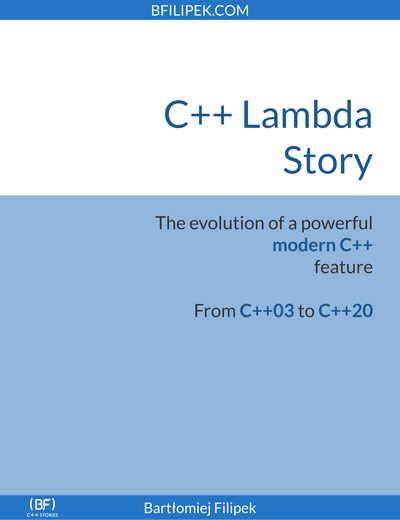
\includegraphics[width=0.9\linewidth]{lambda.png}
		\end{column} \pause
		\begin{column}{0.48\linewidth}
			
\includegraphics[width=0.9\linewidth]{Cpp17.png}
		\end{column}
	\end{columns}
\end{frame}

\begin{frame}{Invitations:}
	\begin{description}[<+->]
		\item [My blog]  \href{blog.panicsoftware.com}{\alert{blog.panicsoftware.com}}
		\item [Cpp Polska] \href{cpp-polska.pl/}{\alert{cpp-polska.pl}}
		\item [Cpp Polska Slack] \href{cpppolska.slack.com}{\alert{cpppolska.slack.com}}
		\item [Bartłomiej Filipek's blog] \href{www.bfilipek.com}{\alert{www.bfilipek.com}}
	\end{description}
\end{frame}

\section{Questions?}

\end{document}